\pagebreak
\restoregeometry 
\section{Modelos de reducción de dimensiones.}

\subsection{Análisis de componentes principales (PCA)}

Al hacer el análisis de componentes principales a los datos se obtuvieron las siguientes cargas en las primeras dos componentes. La varianza acumulada en las primeras dos componentes es del $83.59 \%$ y se considera suficiente para el análisis.
Como se puede observar la primera componente está asociada con la ceniza, el sodio y la proteína, mientras que la segunda se asocia con la humedad, los carbohidratos y las calorías.
Las componentes principales se obtuvieron usando la función \textsf{prcomp} de R con los datos normalizados, la normalización no afectó drásticamente la representación gráfica, sin embargo, permitió observar de forma más clara las relaciones entre las variables ya mencionadas.


\begin{table}[ht]
\centering
\begin{tabular}{rrr}
  \hline
 & PC1 & PC2 \\ 
  \hline
Humedad & 0.21 & 0.58 \\ 
  Proteina & -0.47 & -0.03 \\ 
  Grasa & -0.19 & 0.41 \\ 
  Ceniza & -0.51 & 0.15 \\ 
  Sodio & -0.47 & -0.02 \\ 
  Carbohidratos & 0.32 & -0.49 \\ 
  Calorias & -0.34 & -0.48 \\ 
  Varianza acumulada & 48.64 \% &  83.59 \% \\ 
\end{tabular}
	\label{tabla:pesos_PCA}
	\caption{Pesos asociados a las primeras dos componentes principales.}
\end{table}


\begin{figure}[h]
\centering
	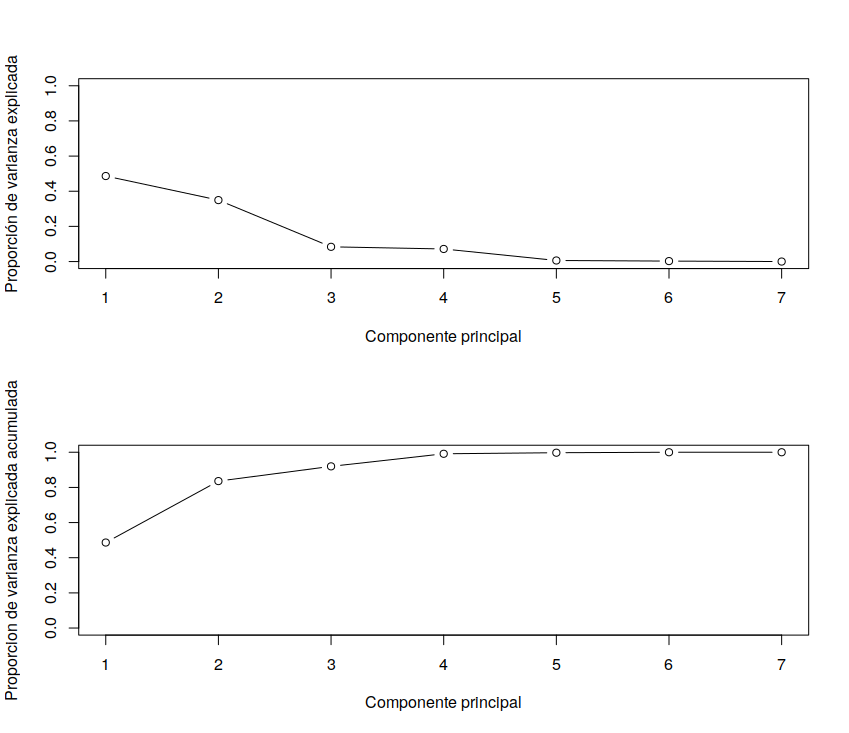
\includegraphics[scale=.5]{images/varPCA.png} 
	\label{i_var_PCA}
	\caption{Varianza explicada por las componentes principales}
\end{figure}

\subsubsection{Representación gráfica (biplot)}

La figura  \ref{i_biplot_PCA} muestra la representación en las primeras dos componentes principales de los datos, en ella se aprecia una clara separación entre algunos grupos de pizzas, específicamente, la marca A se distingue por tener altos niveles de sodio y proteina, las marcas B, C y D se caracterizan por un alto nivel de ceniza, E y F por tener altos valores de humedad, finalmente el resto de marcas (G, H, I, J, K y L) se distinguen por su alto contenido en carbohidratos. 
También el biplot muestra la alta colinealidad existente entre las variables sodio y proteina, y sugiere un contraste entre la variables grasa y carbohidratos.


\begin{figure}[h]
\centering
	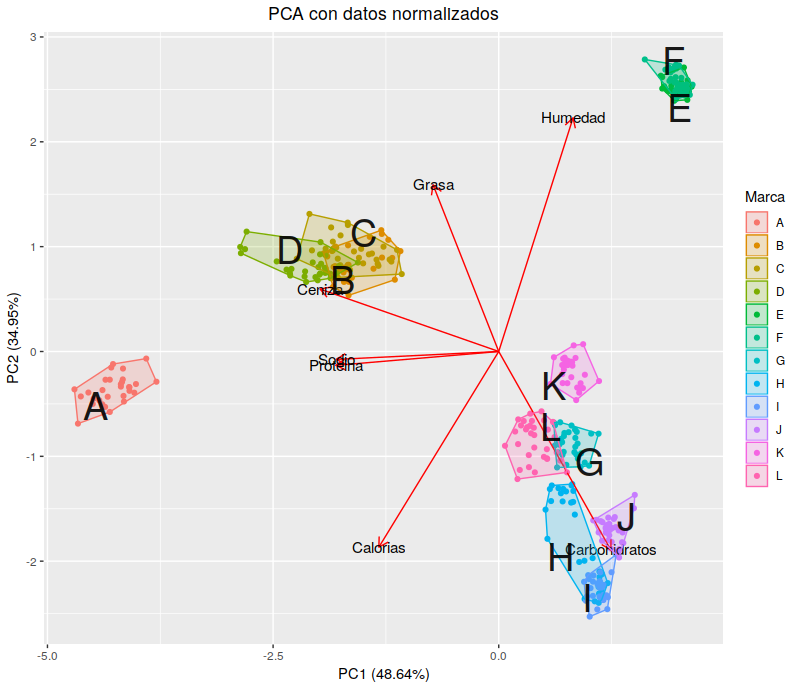
\includegraphics[scale=.75]{images/biplotPCA.png} 
	\label{i_biplot_PCA}
	\caption{Biplot PCA}
\end{figure}


\restoregeometry 
\subsection{Análisis de factores}

Se realizó el análisis de factores usando dos factores, esto debido a la baja dimensión del problema. Para ello se uso la función \textsf{factanal} de R, que estima los factores usando el método de máxima verosímilitud, además, se usó la rotación varimax. \\
El resumen de los resultados se muestra en la tabla \ref{tabla:factores}. El valor del estadístico de prueba $\chi^2$ (con 8 grados de libertad) para verificar la hipótesis nula que la matriz de correlación de datos puede ser representada usando dos factores es $1837.4$, obteniendo además un $p-$valor de 0, por lo que la hipótesis nula se rechaza. Este resultado puede ser explicado por el hecho de que el determinante de la matriz de correlación es cercano a cero. A pesar de ello, se puede afirmar que la aproximación a la matriz de correlación a partir de la matriz $LL' + \Psi$ es adecuada, como se muestra en la tabla \ref{tabla:aproximacion}, la diferencia entre la matriz R y $LL' + \Psi$ es mínima, considerando un redondeo a tres dígitos. Esto en conjunto con el hecho que la proporción de varianza acumulada usando dos factores es del $80.9 \%$, permite afirmar que dos factores son suficientes para la representación de los datos.

\begin{table}[ht]
\centering
\begin{tabular}{rrrrr}
  \hline
 & Factor1 & Factor2 & Varianza específica & Comunalidades \\ 
  \hline
Humedad & 0.06 & -1.00 & 0.01 & 1.00 \\ 
  Proteina & 0.76 & 0.44 & 0.23 & 0.77 \\ 
  Grasa & 0.47 & -0.30 & 0.69 & 0.31 \\ 
  Ceniza & 0.94 & 0.19 & 0.08 & 0.92 \\ 
  Sodio & 0.73 & 0.39 & 0.32 & 0.68 \\ 
  Carbohidratos & -0.90 & 0.44 & 0.01 & 1.00 \\ 
  Calorias & 0.23 & 0.97 & 0.01 & 0.99 \\     
  Proporción de Varianza  & 44 \% &  36.9 \% \\
  Varianza acumulada & 44 \% &  80.9 \% \\ 
   \hline
\end{tabular}
	\label{tabla:factores}
	\caption{Resultados del análisis factorial.}
\end{table}


\begin{table}[ht]
\centering
\begin{tabular}{rrrrrrrr}
  \hline
 & Humedad & Proteina & Grasa & Ceniza & Sodio & Carbohidratos & Calorias \\ 
  \hline
Humedad & -0.00 & -0.02 & 0.00 & -0.00 & 0.01 & -0.00 & -0.00 \\ 
  Proteina & -0.02 & 0.00 & -0.01 & -0.01 & -0.22 & -0.01 & -0.04 \\ 
  Grasa & 0.00 & -0.01 & 0.00 & -0.01 & -0.00 & -0.00 & 0.00 \\ 
  Ceniza & -0.00 & -0.01 & -0.01 & -0.00 & 0.06 & 0.00 & -0.00 \\ 
  Sodio & 0.01 & -0.22 & -0.00 & 0.06 & -0.00 & 0.01 & 0.04 \\ 
  Carbohidratos & -0.00 & -0.01 & -0.00 & 0.00 & 0.01 & -0.00 & -0.00 \\ 
  Calorias & -0.00 & -0.04 & 0.00 & -0.00 & 0.04 & -0.00 & 0.00 \\ 
   \hline
\end{tabular}
	\label{tabla:aproximacion}
	\caption{Diferencia entre R y $LL' + \Psi$, con redondeo a tres dígitos.}
\end{table}

\subsubsection{Interpretación}

El primer factor se relaciona principalmente con las variables ceniza, carbohidratos y proteina mientras que el segundo factor se asocia con la humedad y las calorías. Las varianzas específicas y las comunalidades indican que la varianza de la mayoría de las variables queda bien explicada a partir de los factores, con excepción de la variable grasa, cuya varianza específica es de $.69$.

\subsubsection{Representación gráfica (biplot)}

Para obtener una representación gráfica en dos dimensiones, se realizó la estimación de los \textit{scores} usando el método de Bartlett. El biplot resultante se muestra en la figura \ref{i_biplot_Factores}. El resultado es muy similar al obtenido usando componentes principales, pues se logran diferenciar los mismos grupos que las marcas forman de acuerdo a sus características; sin embargo, existe una pequeña diferencia y es que las marcas K y L se separan del grupo formado por las marcas G, H, I y J, para situarse más al centro de la gráfica, lo que indica que los niveles de nutrientes de las marcas K y L se situán cerca de la media.

\begin{figure}[h]
\centering
	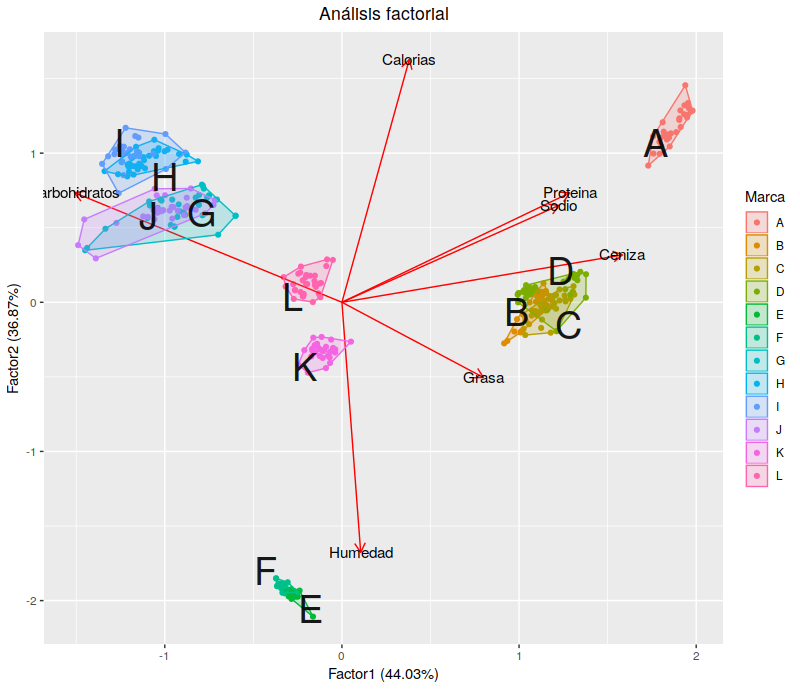
\includegraphics[scale=.75]{images/biplotFactores.png} 
	\label{i_biplot_Factores}
	\caption{Biplot usando 2 factores}
\end{figure}